\documentclass[12pt]{report} % The command
% [12pt] : sets the font size to 12 pt
% Latex ma default font size: about 10-11


\usepackage{parskip}
% \usepackage[a4paper, margin=1in]{geometry}

% To control the geomertry of paper: size , margin
\usepackage[a4paper,inner=1.5in, outer=1in, top=1in, bottom=1in]{geometry}
% curly bracket bhitra : Compulsory parameters
% big bracket bhitra: Optional parameters.

\usepackage{times} % changing font to times new roman.


% For Underline error fix
\usepackage{soul} % gives \ul{}


% For mathematical typesetting
\usepackage{amsmath, amssymb, amsfonts}

% for times new roman math font
\usepackage{mathptmx}

% for images
\usepackage{graphicx}

\usepackage{float}

\setlength{\parskip}{1em}
\begin{document} % The environment
% The content area.
\begin{titlepage}
    \centering % equivalent to scoped centerign using \begin{center}  \end{center}
    % adding figure without using \begin{figure}
    
\includegraphics[width=7cm]{figures/tulogo.png}\\
    TRIBHUVAN UNIVERSITY\\
    INSTITUTE OF ENGINEERING\\
    PULCHOWK CAMPUS\\
    \vfill % divides the page space with no. of vfills used.
    % \vskip also available re or \vspace{2cm}: To give spacing
    SOME PROJECT REPORT\\
    \vfill
    SUBMITTED BY\\
    ME
    % ALIZ BHATTARAI & (082BCT008)
    % \\
    % ABHISHEK THAGUNNA & (082BCT007)
    \vfill
    SUBMITTED TO\\
    DEPARTMENT OF COMPUTER ENGINEERING\\
    \vfill
    12 AUGUST, 2026
    
\end{titlepage}
\pagenumbering{roman} % using Roman -> Makes the numering capitalized roman
\chapter*{Copyright}
\chapter*{Abstract}
My first (self-written) Latex Dcoument. 

\tableofcontents
\chapter{Introduction}
\pagenumbering{arabic} % using arabic format numbering from this page forward
    \section{Background}
         \subsection{History}

The afternoon sun filtered through the dense canopy of ancient oaks, casting shifting patterns of light and shadow across the forest floor. A gentle breeze rustled the leaves, carrying the earthy scent of damp moss and pine needles. Somewhere in the distance, a stream murmured softly over smooth river stones, providing a tranquil soundtrack to the quiet wilderness.

Urban planning has undergone a dramatic transformation over the past decade, heavily influenced by the push for environmental sustainability. City architects now prioritize green roofs, extensive bike lane networks, and energy-efficient public transit systems over car-centric infrastructure. These changes not only reduce carbon footprints but also significantly improve the overall quality of life for urban residents.

% \\ : New line
% \\ and enter (space between lines) : paragraph space also gives
Culinary arts require a delicate balance of precision, creativity, and sensory awareness. A master chef does not merely follow a recipe; they understand the chemistry of flavor combinations, how heat alters molecular structures, and the importance of presentation. Every dish tells a story, reflecting cultural heritage and personal passion on a plate.

Deep beneath the ocean's sunlit surface \ul{lies a mysterious realm where sunlight never reaches. In this crushing pressure and perpetual darkness, $x^{24}+3x_{32}+5$ bizarre creatures thrive through biological adaptations like bioluminescence. Giant tube worms, anglerfish, and ghostly white octopuses navigate hydrothermal vents that spew superheated, mineral-rich water into the abyss.}\\
..\\
$\alpha \beta \gamma \theta \nu \pi \xi \zeta \delta \Delta \lambda \Lambda $

The digital revolution has fundamentally altered how humans communicate, consume information, and form relationships. Social media platforms connect individuals across \[\text{Acceleration of a car}=\dfrac{dx}{dt}\]vast geographical distances in milliseconds, creating global communities centered around niche interests. However, this hyper-connectivity also presents modern challenges regarding privacy, attention spans, and the digital divide.

\[Acceleration\ of\ a\ car=\dfrac{dx}{dt}\] % somewhat my trick : escaping a trick
\[\text{Acceleration of a car}=\dfrac{dx}{dt}\] % better option
\vfill

\[\text{Acceleration of a car}=(\dfrac{dx}{dt})\] % well not as we wanted.
\[\text{Acceleration of a car}=\left( \dfrac{dx}{dt}\right)\] 
\vfill

\[\text{Acceleration of a car}=\left( \dfrac{dx*1/2}{dt}\right)\] 
\[\text{Acceleration of a car}=\left( \dfrac{dx\times\dfrac{1}{2}}{dt}\right)\] % to have brackets as desired
\vfill
\[\text{Acceleration of a car}=\left( \dfrac{\partial x\times\dfrac{1}{2}}{\partial t}\right)\] 
\[\text{Acceleration of a car}=\int\left( \dfrac{dx\times\dfrac{1}{2}}{dt}\right)\] 
\vfill
\[\text{Acceleration of a car}=\prod\left( \dfrac{dx\dfrac{1}{2}}{dt}\right)\] 
\[\text{Acceleration of a car}=\prod_{0}{\infty}\left( \dfrac{dx\times\dfrac{1}{2}}{dt}\right)\] 
\vfill
\[\text{Acceleration of a car}=\sum\left( \dfrac{dx\times\dfrac{1}{2}}{dt}\right)\] 
\[\text{Acceleration of a car}=\sum_{0}{\infty}\left( \dfrac{dx\times\dfrac{1}{2}}{dt}\right)\] 
\[\text{Acceleration of a car}=\lim\left( \dfrac{dx\times\dfrac{1}{2}}{dt}\right)\] 
Whispered legends speak of an abandoned railway tunnel tucked away in the forgotten hills, swallowed entirely by ivy and creeping vines. Locals avoid the area after sundown, claiming to hear the distant screech of iron wheels and a lonely locomotive whistle echoing through the valley. Whether these tales are mere folklore or echoes of history remains a subject of endless debate.

Astronauts aboard the International Space Station experience a perspective shift known as the overview effect. Gazing down at Earth from orbit reveals a vibrant, fragile blue marble suspended in the vast, indifferent void of space, devoid of visible political borders. This profound vantage point inspires a deep sense of global stewardship and interconnectedness among those fortunate enough to witness it.

Artisanal pottery is an ancient craft that demands immense patience and respect for the medium. Transforming a lump of raw clay into a functional vessel involves meticulous wedging, centering on the potter's wheel, shaping, trimming, and multiple rounds of firing in a kiln. Each finished piece carries subtle imperfections that reveal the physical touch of its creator.

The art of storytelling has been a cornerstone of human civilization since the days of cave paintings and oral traditions around flickering campfires. Whether expressed through novels, cinema, or immersive digital media, compelling narratives tap into universal emotions and psychological archetypes. They allow us to walk in another's shoes and make sense of a complex world.

Meticulous preparation is the bedrock of any successful archaeological expedition. Researchers spend months analyzing satellite imagery, historical archives, and geological maps before ever setting foot in the field. When excavation finally begins, every artifact must be meticulously documented, measured, and preserved to unlock the silent secrets of bygone eras.
\subsection{Context}
                %  \subsubsection{The Reason Why This Exists}
    % This enumerates in numbered way. (Ordered list)
    \begin{enumerate}
    \item{One}
    \item{Two}
    \item{Three}
        \begin{enumerate}
            \item{sub-one}
            \item{sub-two}
            \item{sub-three}
                \begin{enumerate}
                    \item{sub-sub-one}
                    \item{sub-sub-two}
                    \item{sub-sub-three}
                \end{enumerate}
        \end{enumerate}
    \end{enumerate}
    \section{Problem Statement}

    % Bullet point like Itemization (unordered List)
    \begin{itemize}
    \item{One}
    \item{Two}
    \item{Three}
        \begin{itemize}
            \item{sub-one}
            \item{sub-two}
            \item{sub-three}
                \begin{itemize}
                    \item{sub-sub-one}
                    \item{sub-sub-two}
                    \item{sub-sub-three}
                \end{itemize}
        \end{itemize}
    \end{itemize}
    \section{Objective}
    \section{Scope of Study}
    \section{Limitation}


     \begin{eqnarray}
        x^2+2x&=&3 \nonumber\\
        x^2 &=&3-2x \nonumber
    \end{eqnarray}
    
    \section{Study Area}
    
    \begin{equation}
        \lim_{x to \infty}\left(\dfrac{x^2-2}{x-2}\right)
    \end{equation}

    \begin{eqnarray}
        x^2+2x&=&3 \\
        x^2 &=&3-2x
        % C = \begin{bmatrix}
        %     1 & 2 & 3 \\
        %     4 & 5 & 6
        % \end{bmatrix}
    \end{eqnarray}

    \begin{eqnarray} 
    A = \begin{Bmatrix}
        1 & 2 & 3\\
        4 & 5 & 6 \\
        7 & 8 & 9
    \end{Bmatrix}\\
    \\
    C = \begin{Bmatrix}
        1 & 2 &\hdots &3\\
        4 & 5 &\hdots & 6 \\
        7 & 8 &\hdots & 9
    \end{Bmatrix}\\
    \\
    D = \begin{Bmatrix}
        1 & 2 &\vdots &3\\
        4 & 5 &\vdots & 6 \\
        7 & 8 &\vdots & 9\\
        \vdots & \vdots &\vdots & \vdots\\
        10 & 11 & 12 & 13
    \end{Bmatrix}\\
    \\
    B = \begin{pmatrix}
        1 & 2 & 3 \\
        4 & 5 & 6 \\
        7 & 8 & 9
    \end{pmatrix}\\
    \\
    E = \begin{Bmatrix}
        1 & 2 &\ddots &3\\
        4 & 5 &\ddots & 6 \\
        7 & 8 &\ddots & 9
    \end{Bmatrix}\\
    \end{eqnarray}
     \[\sqrt[4]{\dfrac{x^2+2x+5}{2}}\quad \sin \theta \log5\]
   
    \begin{equation}
        f(x) =  \begin{cases}
            x^2-2 & \text{for } x \leq 0 \\
            x & \text{for } x > 0
        \end{cases}
    \end{equation}
\chapter{Literature Review}
\section{Figures}

% This figure env for the caption and numbering of figures.
% image can be added without this.
\begin{figure}[h]  % h to specify here (don't go stranding other place)
    \centering
    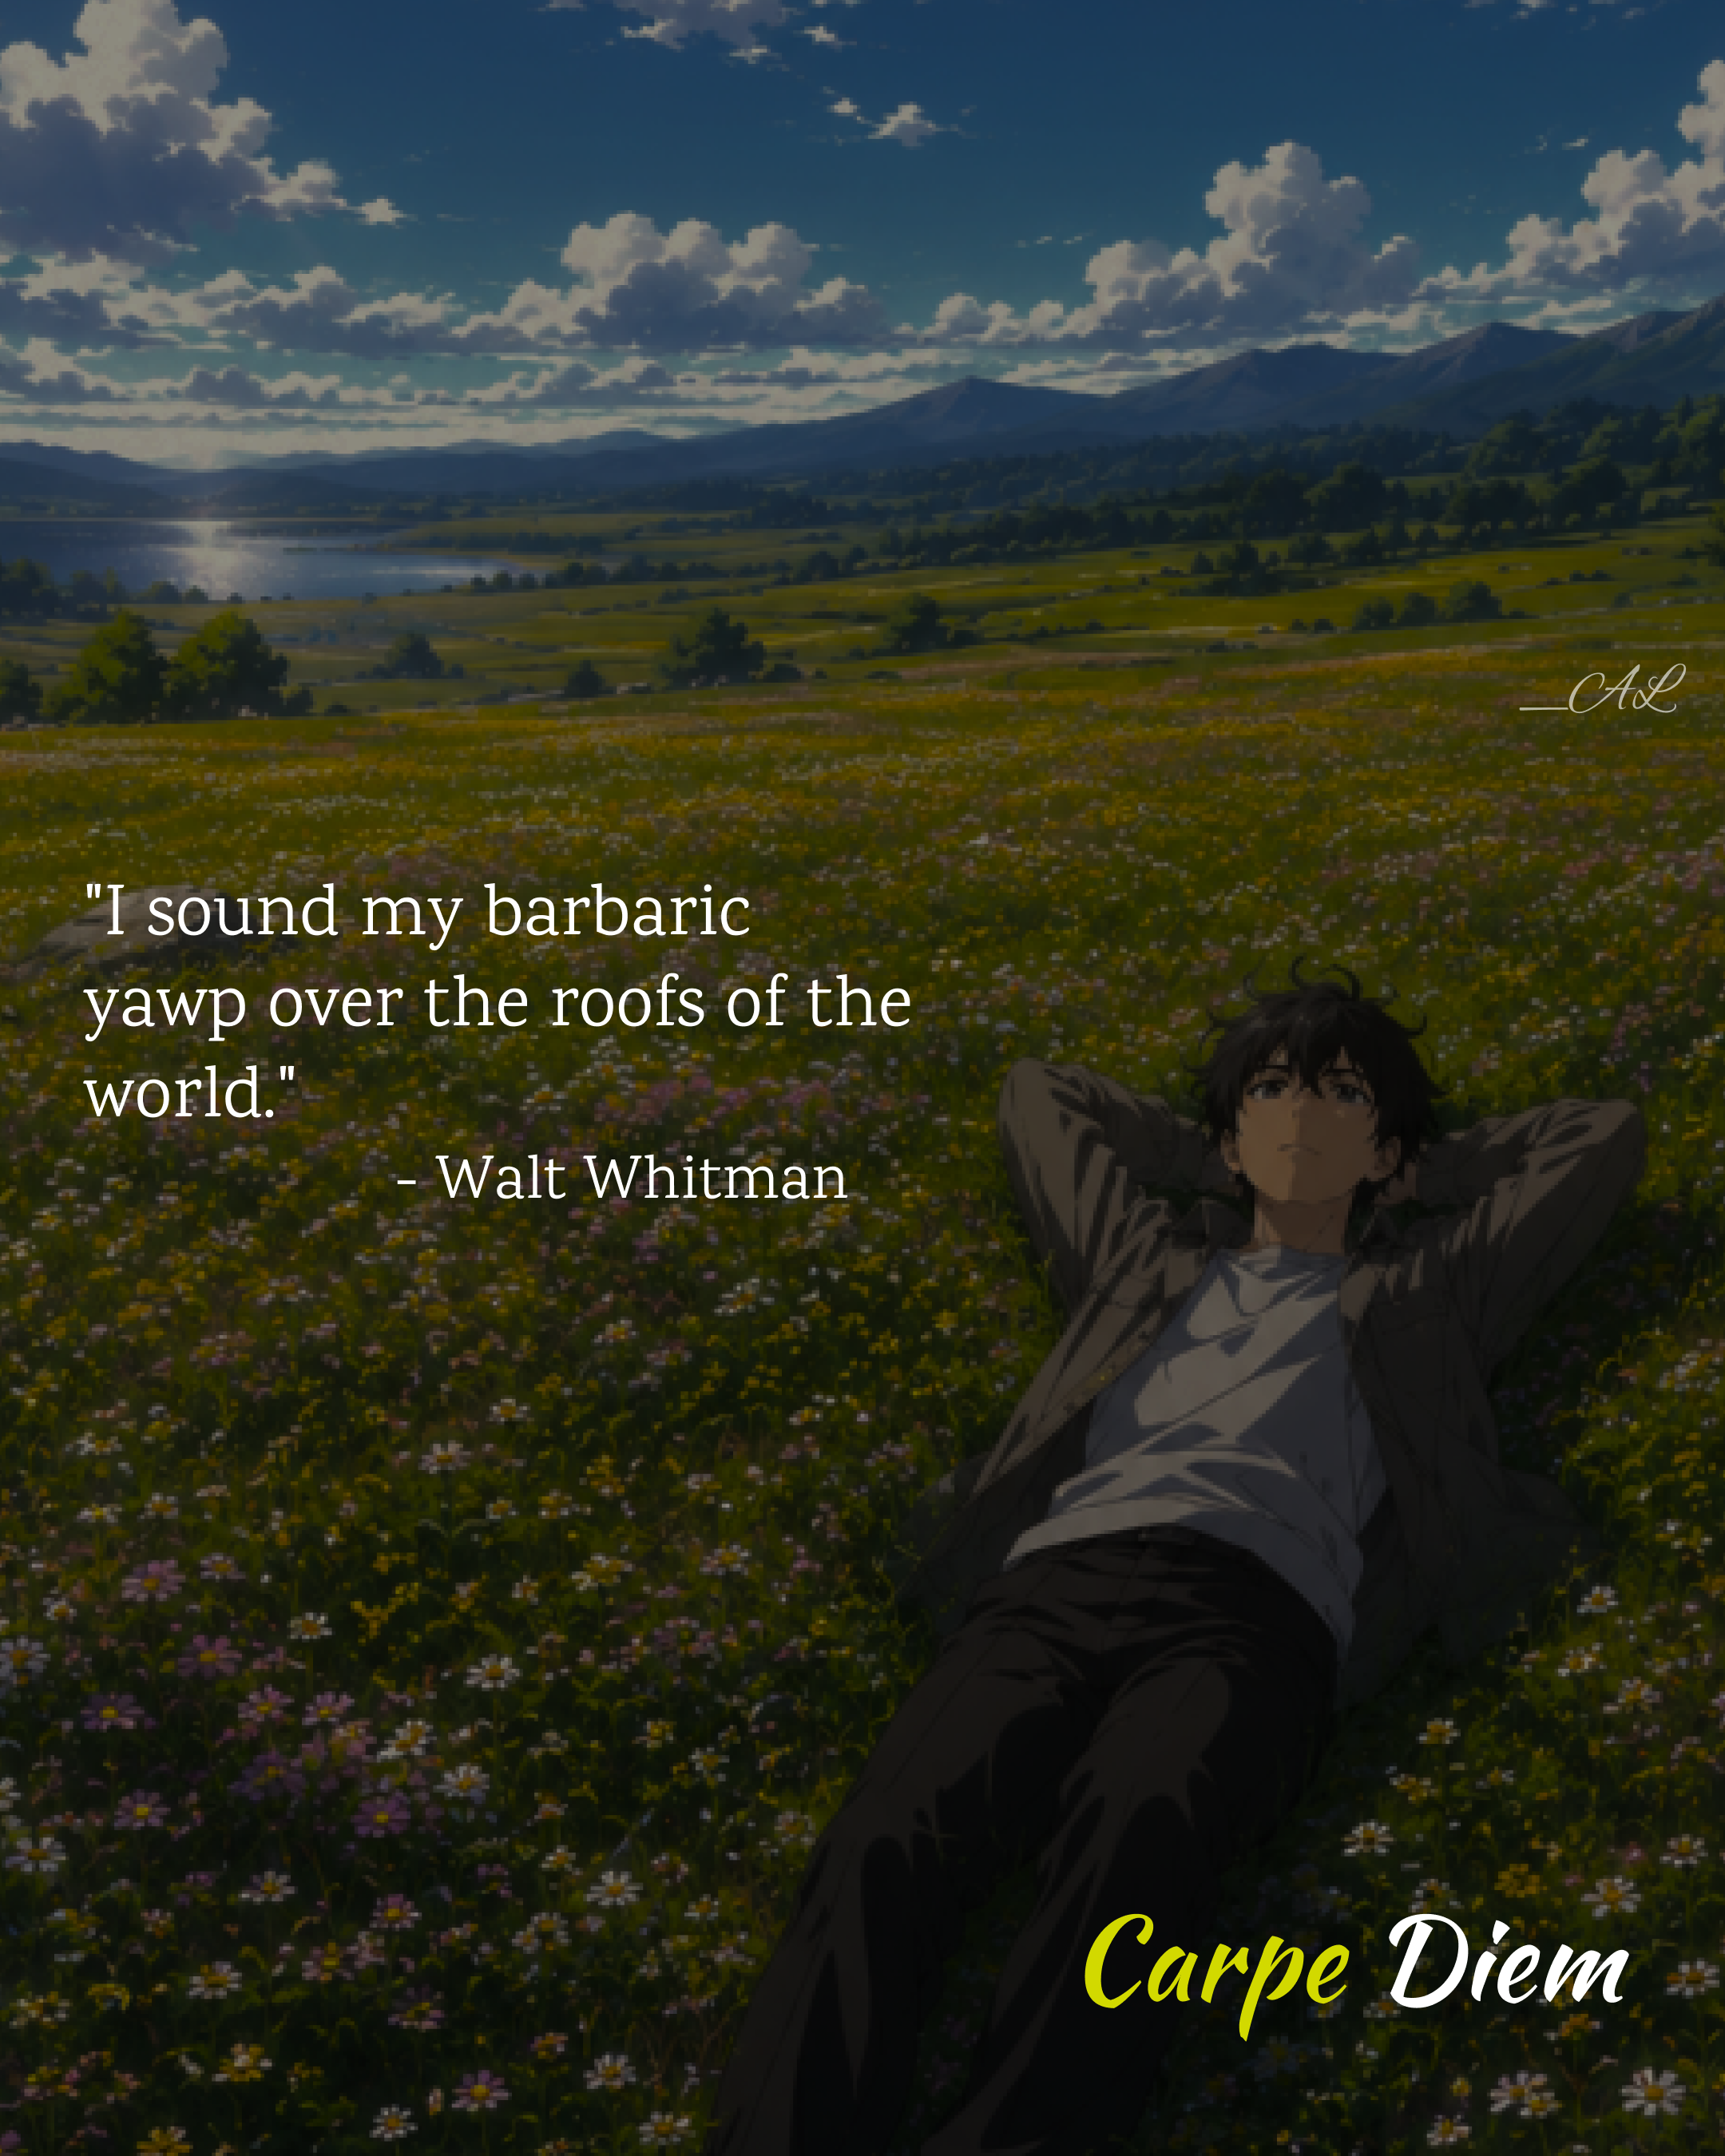
\includegraphics[width=0.6\textwidth]{figures/ForTrial.png}
    \caption{`Carpe Diem`}
    \label{fig:My Trial}
\end{figure}

% h (here) , t (next page top), b (bottom of next page)
% tries to keep the image here or t or b
% using htb tries the following: try here, or next page's top or next page bottom.
% Using H is forcing the image to be fixed at that place
% kinda distorts page order / content order
% To use H package float is required.

% \linewidth also exists.
% \textwidth for the entire text length or smth.
\chapter{Methodology}
\section{Table}{
    
}
\chapter{Result and Discussion}
\chapter{Conclusion}
    \section*{Unnumbered Section} % * removes the numbering
\end{document}